\documentclass[11pt,xcolor={dvipsnames},aspectratio=159,hyperref={pdftex,pdfpagemode=UseNone,hidelinks,pdfdisplaydoctitle=true},usepdftitle=false]{beamer}
\usepackage{presentation}[aspectratio=169]
\usepackage{math}
\usepackage{mathtools}
\usepackage{mleftright}
\usepackage{algorithm}% http://ctan.org/pkg/algorithms
\usepackage{algpseudocode}% http://ctan.org/pkg/algorithmicx
\hypersetup{
    colorlinks=magenta,
    linkcolor=magenta,
    filecolor=magenta,      
    urlcolor=magenta,
    }
% Enter title of presentation PDF:

% Enter title of presentation PDF:
\hypersetup{pdftitle={Optimization}}
% Enter link to PDF file with figures:


\begin{document}
% Enter presentation title:
\title{Optimization}
\subtitle{Quantitative Economics 2024}
% Enter presentation information:

% Enter presentation authors:
\author{Piotr Żoch}%
% Enter presentation location and date (optional; comment line if not needed):
\frame{\titlepage}

% Fill out content of presentation:
\begin{frame}{Optimization in economics}   
\begin{itemize}
    \item Economics: agents \al{optimize} subject to constraints
\begin{itemize}
    \item Maximize utility subject to budget constraints
    \item Minimize expenditure to attain a given level of utility
    \item Maximize profits subject to consumer demand
    \item Minimize costs of production subject to available technology
\end{itemize}
\item Optimization also used in \al{estimation} -- find parameters that minimize some loss function / maximize likelihood.
\end{itemize}
\end{frame}


\begin{frame}{Optimization}
The most general minimization problem is
   \begin{align*}
         \min_{\bm{x}} \quad & \al{f}\bp{\bm{x}} \\
        \text{s.t. } \quad & \alg{\bm{g}}\bp{\bm{x}} = 0 \\
        & \alb{\bm{h}}\bp{\bm{x}} \leq 0
   \end{align*}
where \al{$f : \R^n \rightarrow R$} is the \al{objective} function, \alg{$\bm{g}: \R^n \rightarrow \R^m$} is the vector of \alg{$m$ equality constraints}, and \alb{$\bm{h}: \R^n \rightarrow \R^l$} is the vector of \alb{$l$ inequality constraints}.
\vspace{1cm}

Note: \al{maximization} problem can be converted to a minimization problem by multiplying the objective by $-1$.

\end{frame}
\begin{frame}{Words of wisdom}

    \begin{itemize}
        \item Optimization is difficult!
        \item \emph{Never} reinvent the wheel! Understand some basics about the main algorithms, but use existing packages to solve your problems.
        \item No free lunch theorem by Wolpert and Macready (1997) -- \al{no optimization algorithm is better than any other algorithm on all problems}.
        \item Be careful: try to understand what you are doing and what the algorithm is doing. 
        \item Never be happy: always check if the algorithm converged, if the solution makes sense, if the solution is robust to changes in starting points, etc.
    \end{itemize}

\end{frame}

\begin{frame}{Algorithms}
    \begin{itemize} 
    \item All numerical optimization algorithms -- same idea: search through the space of feasible choices to find the best one. The difference is in how they search.
    \begin{itemize}
        \item \alb{Comparison methods}: compute the objective function at a finite number of points and choose the best one. No need for derivatives etc.
        \item \alg{Gradient methods}: use information about the gradient of the objective function and constraints to guide the search.
        \item \alr{Curvature methods}: use also information about the curvature of the objective function and constraints.
    \end{itemize}    
\alb{Comparison methods} do not require strong conditions, but they are slow. \alr{Curvature methods} are fast, but require strong conditions.
\end{itemize}
\end{frame}

\begin{frame}
    \heading{Unidimensional optimization}
    \end{frame}

    \begin{frame}{Bracketing methods}
        \begin{itemize}
        \item A \alg{derivative-free} method for \al{univariate} $f$.
\item Works \al{only} on \alb{unimodal} function $f$ -- otherwise it can converge to a local minimum.
\item We can find a bracket in which the global minimum exists if we can find points $a < z < b$ such that
$$f(a) \geq f(z) < f(b) \text{ or } f(a) > f(z) \leq f(b)$$
\item Bracketing methods differ in how:
\begin{enumerate}
\item they choose the initial bracket;
\item they shrink the bracket.
\end{enumerate}
        \end{itemize}
\end{frame}

\begin{frame}{Bracketing methods}
    \begin{itemize}
\item \alg{Golden section search}: two function evaluations are made at the first iteration and
then only one function evaluation is made for each subsequent iteration. Bracket shirnks by a constant factor $\phi \approx 1.618$ (golden ratio).
\item \alr{Fibonacci search}: bracket shrinks by a factor $\frac{F_{n-1}}{F_n}$, where $F_n$ is the $n$-th Fibonacci number.
\item   For a large number of iterations, the two methods are equivalent.    
\end{itemize}
  
\end{frame}

\begin{frame}{Bracketing methods}
    \centering
    \begin{figure}
    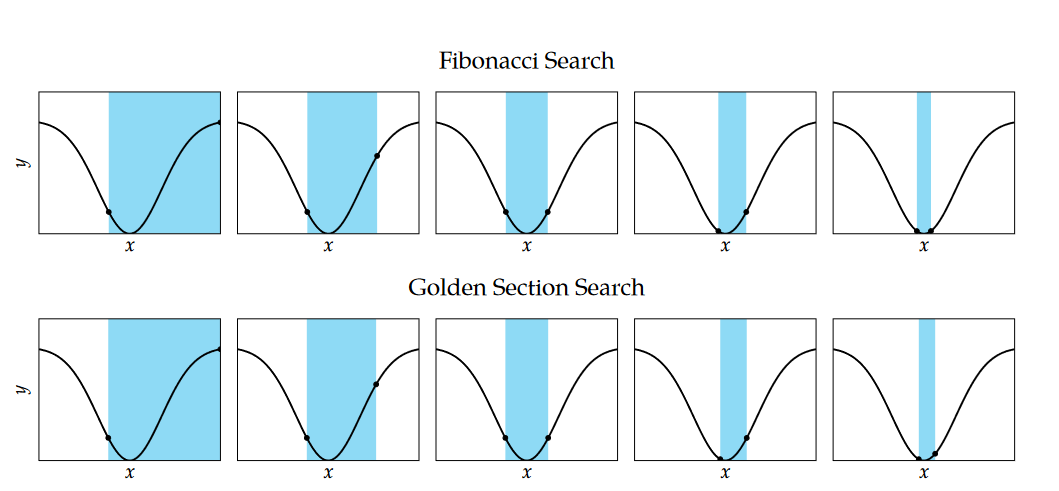
\includegraphics[width=1\textwidth]{bracketing.png}
    \caption{Source: \href{https://mitpress.mit.edu/9780262039420/}{Kochenderfer and Wheeler (2019)}}
    \end{figure}
\end{frame}


\begin{frame}{Golden section search}
    \begin{itemize}
        \item Focus on the bracket $[a,b]$.
\item Constant reduction factor $c$: \begin{align*}
b_{n+1} - a_{n+1} &= c\bp{b_n - a_n}
\end{align*}
        \item We start with a bracket $\bs{a_0,b_0}$.
\item We initialize by evaluating $f$ at two points: $x_1 < x_2$ inside the bracket.
\item If $f\of{x_1} < f\of{x_2}$, we set $b_1 = x_2$:  \begin{align*}
    x_2 =  \bp{1-c} a_1 + c b_1
\end{align*}
\item Otherwise, we set $a_1 = x_1$: \begin{align*}
    x_1 = b_1 + c \of{b_1 - a_1}
\end{align*}
\end{itemize}
  
\end{frame}


\begin{frame}{Golden section search}
    \begin{itemize}
        \item If we know $c$ we know how to update brackets. 
        \item How to choose $c$?
        \item Assume for simplicity that the length of the bracket is $1$ and $f\of{x_1}<f\of{x_2}$.
        \item We then have a new bracket $[0,x_2]$, where $x_2 = c$ and $x_1 = 1-c$.
        \item In the next iteration we reuse $f\of{x_1}$ and evaluate $f$ at a \al{new} point $x_2$.
        \item Is $x_1<x_2$ or $x_1>x_2$? Let us consider both cases. 
\end{itemize}
\end{frame}


\begin{frame}{Golden section search}
    \begin{itemize}
        \item Suppose $x_1<x_2$.
        \item $x_1$ satisfies two conditions: \begin{align*}
            x_1 =&  1 - c \\
            x_1 =&  c \bp{1-c}
        \end{align*}
        \item This implies $\bp{1-c}^2 =0$ with solution $c=1$.
        \item But this is useless -- $c=1$ means that we do not shrink the bracket at all.
\end{itemize}
\end{frame}

\begin{frame}{Golden section search}
    \begin{itemize}
        \item Suppose $x_2<x_1$.
        \item $x_1$ satisfies two conditions: \begin{align*}
            x_1 =&  1- c \\
            x_1 =&  c^2
        \end{align*}
        \item This implies $c^2 +c -1 =0$ with a positive solution $c=\frac{-1+\sqrt(5)}{2}$. We take it as $c$.
        \item $1+c = \frac{1+\sqrt{5}}{2} = \phi$ -- the \al{golden ratio}.
\end{itemize}
\end{frame}

\begin{frame}{Newton's Method}

\begin{itemize}
    \item Let $x_0$ be a point. We can approximate the objective function $f$ by a quadratic function $p\of{x}$ around $x_0$: 
    $$ p\bp{x} \equiv f\bp{x_0} + f^\prime\bp{x_0} \bp{x-x_0} + \frac{f^{\prime\prime}\of{x_0}}{2} \bp{x-x_0}^2$$ 
    \item The minimum of $p\of{x}$ is at $x_1 = x_0 - \frac{f^\prime\of{x_0}}{f^{\prime\prime} \of{x_0}}$.
    \item We can repeat this procedure to get $x_2, x_3, \dots$, hoping that we will get closer to the extremum of $f$.

    
    \item To summarize:

    \begin{enumerate}
        \item Start at $x_0$
        \item Compute $x_{n+1} = x_n - \frac{f^\prime\of{x_n}}{f^{\prime\prime} \bp{x_n}}$
        \item Stop when $f^\prime\of{x_n} \approx 0$
    \end{enumerate}
    \end{itemize}
    \end{frame}


\begin{frame}{Newton's Method}
    \begin{itemize}
        \item Newton's method is a \al{curvature method} -- it uses information about the curvature of the objective function.
        \item Requires the objective function to have both a continuous first derivative and a continuous second derivative ($C^2$).
        \item \al{Fast} -- \alg{quadratic convergence} in the neighborhood of the optimum.
        \item \al{Not robust} -- it can fail to converge if the starting point is not close enough to the solution.
        \item \al{Local} -- it can converge to a local minimum.
    \end{itemize}
    \end{frame}

    \begin{frame}{Newton's Method}
        \centering
        \begin{figure}
            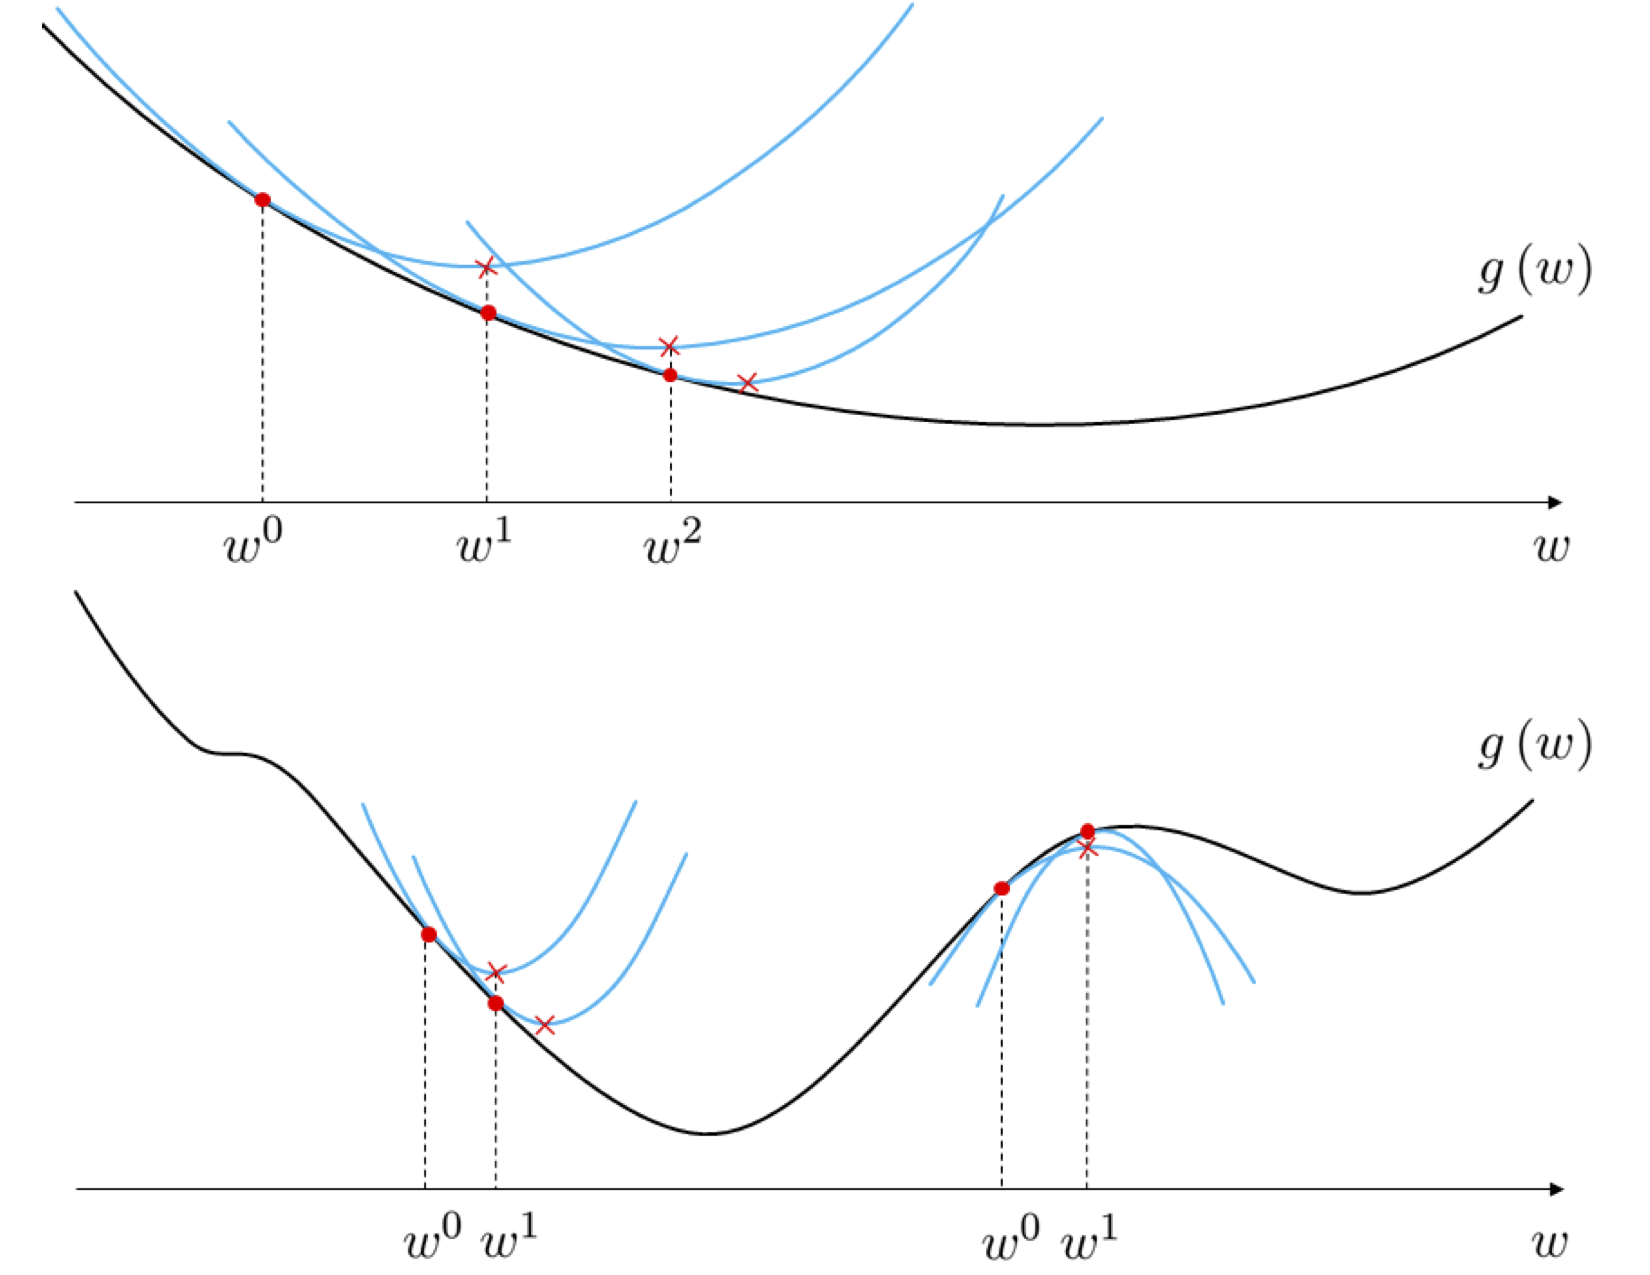
\includegraphics[width=0.6\textwidth]{newton.png}
            \caption{Source: \href{https://jermwatt.github.io/machine_learning_refined/notes/4_Second_order_methods/4_4_Newtons.html}{here}}
            \end{figure}
        \end{frame}


    \begin{frame}{Newton's Method}
        \centering
        \begin{figure}

        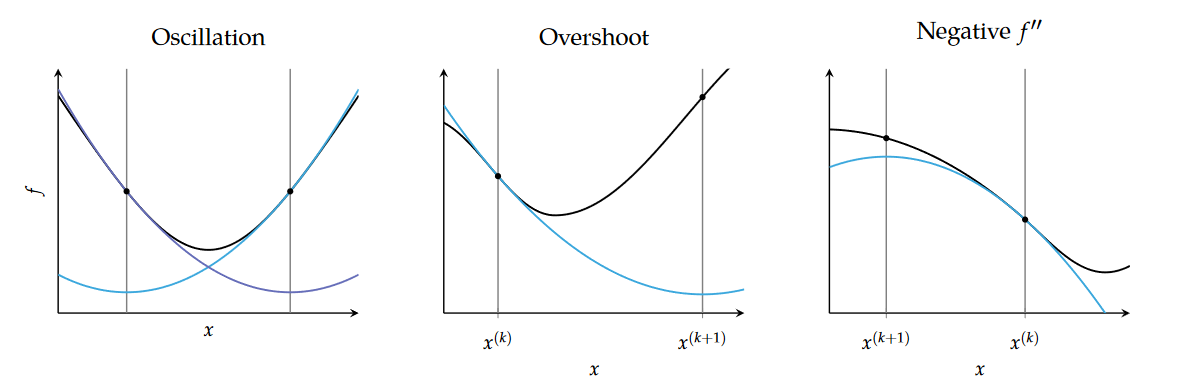
\includegraphics[width=1\textwidth]{newton_failure.png}
        \caption{Source: \href{https://mitpress.mit.edu/9780262039420/}{Kochenderfer and Wheeler (2019)}}
        \end{figure}

    \end{frame}  


    \begin{frame}{Quadratic convergence}
        \begin{theorem}
            Suppose $f\bp{x}$ is minimized at $x^*$, $C^3$ in the neighborhood of $x^*$, and that $f^{\prime\prime}\bp{x^*} \neq 0$. 
            
            Then there exists $\varepsilon > 0$ such that if $\abs{x_0 - x^*} < \varepsilon$, the sequence $$x_{n+1} = x_n - \frac{f^\prime\bp{x_n}}{f^{\prime\prime} \bp{x_n}}$$ converges to $x^*$.
            
            Moreover $$\lim_{n \rightarrow \infty} \frac{\abs{x_{n+1} - x^*}}{\abs{x_n - x^*}^2} = \frac{1}{2} \abs{\frac{f^{\prime\prime\prime}\bp{x^*}}{f^{\prime\prime}\bp{x^*}}}$$ is the quadratic order of convergence.
            \end{theorem}
        \end{frame}

    \begin{frame}{Stopping criterion}
        
        \begin{itemize}
            \item We want to stop when $f^\prime\bp{x_n} \approx 0$. 
            \item In practice, we stop when $\abs{f^\prime\bp{x_n}} < \delta$ for some small $\delta$. But this is not enough! 
            \item If $\abs{f^{\prime\prime}\bp{x_n}}$ is close to zero, the function is flat -- many points with similar $f^\prime$.
            \item Stop if \al{both} $\abs{f^\prime\bp{x_n}} < \delta$ \al{and} $x_n$ and $x_{n+1}$ are close.
            \item Be careful: $\abs{x_{n+1} - x_n}=0.0000001$ means something different if $x_n=100$ and if $x_n=0.0000001$!
            \item Judd (1998) suggest stopping when 
            $$ \abs{f^\prime\bp{x_n}} < \delta \quad\text{and}\quad \abs{x_{n+1} - x_n} < \varepsilon\bp{1+ \abs{x_n}}.$$
        \end{itemize}
        \end{frame}


    \begin{frame}{Brent's Method}
        \begin{itemize}
            \item Combine a slow (but robust) bracketing method with a fast (but not robust) method.
            \item Start with a bracket $[x_0,x_1]$ and find $x_2$ with GSS.
            \item Now you have three points -- find coefficents of the quadratic function that goes through them.
            \item You know how find the minimum of a quadratic function -- this is our $x_3$.
            \item If points are colinear (so that the quadratic function is flat), make a GSS step and try again.
            \item Pick a new bracket (discard one point) and repeat.

        \end{itemize}
    \end{frame}


    \begin{frame}{Brent's Method}
        \centering
        \begin{figure}
            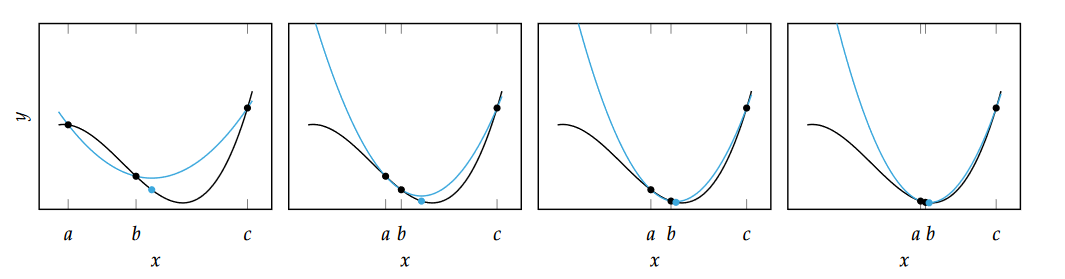
\includegraphics[width=1\textwidth]{quadratic.png}
            \caption{Source: \href{https://mitpress.mit.edu/9780262039420/}{Kochenderfer and Wheeler (2019)}}
        \end{figure}
        \end{frame}

        
    \begin{frame}
        \heading{Multidimensional optimization}
    \end{frame}

    \begin{frame}{Polytope method (Nelder-Mead)}
        \begin{itemize}
        \item Amoeba crawling downhill.
        \item Start with a \alg{simplex} (triangle in 2D, tetrahedron in 3D, etc.) and move it downhill.
        \item Find the worst point and:
        \begin{enumerate}
            \item Reflect it through the centroid of the other points.
            \item If the reflected point is better than the second worst point, try to expand the simplex in that direction.
            \item If the reflected point is worse than the second worst point, try to contract the simplex.
            \item If the reflected point is worse than the worst point, try to contract the simplex towards the best point.
        \end{enumerate}
        \end{itemize}
    \end{frame}

    \begin{frame}{Polytope method (Nelder-Mead)}
        \centering
        \begin{figure}

        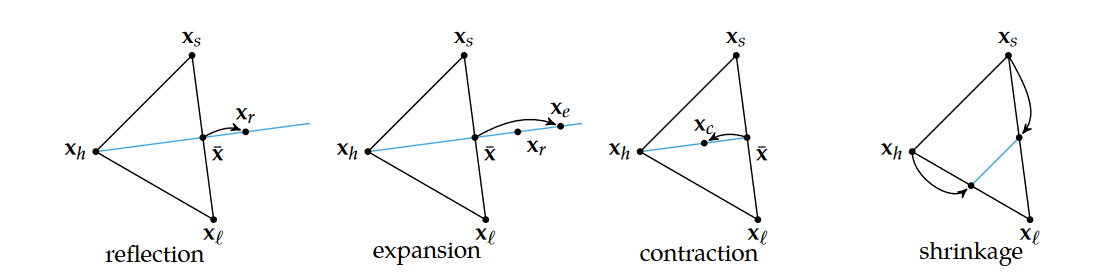
\includegraphics[width=0.95\textwidth]{nelder_mead.png}
        \caption{Source: \href{https://mitpress.mit.edu/9780262039420/}{Kochenderfer and Wheeler (2019)}}
        \end{figure}
    \end{frame}

    \begin{frame}{Polytope method (Nelder-Mead)}
        \centering
        \begin{figure}

        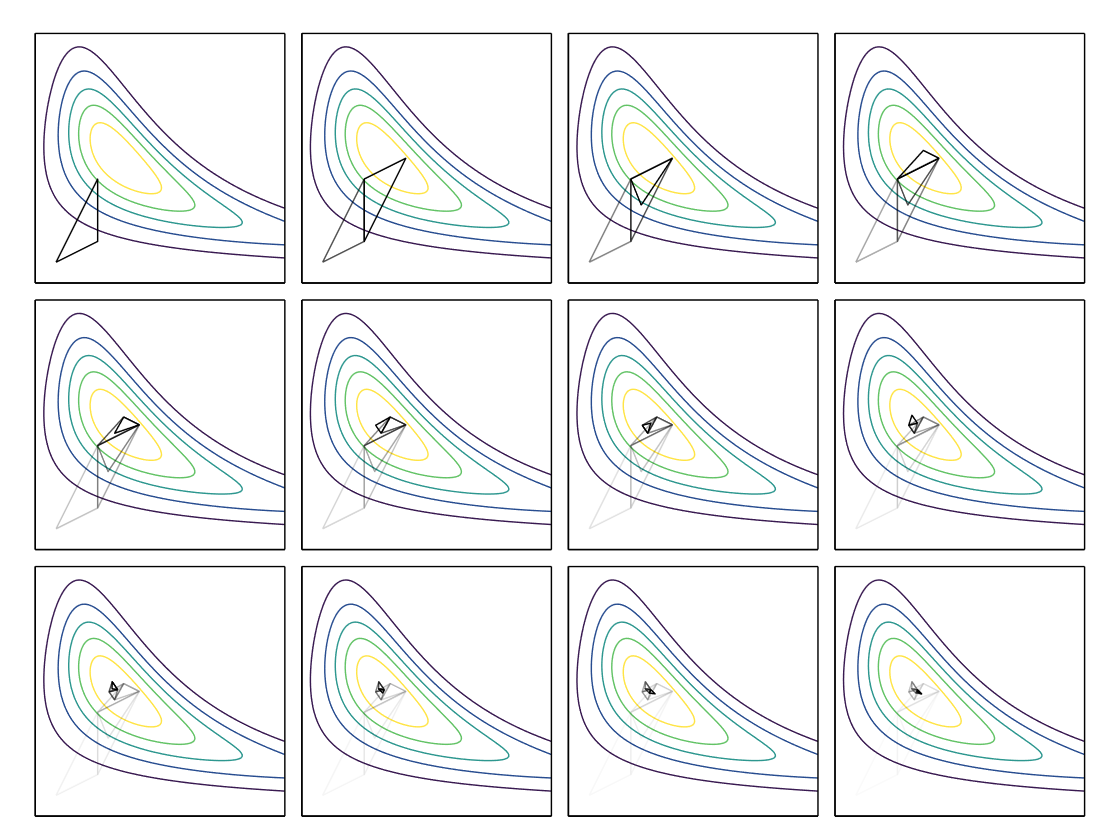
\includegraphics[width=0.6\textwidth]{nelder_mead2.png}
        \caption{Source: \href{https://mitpress.mit.edu/9780262039420/}{Kochenderfer and Wheeler (2019)}}
        \end{figure}
    \end{frame}

    \begin{frame}{Polytope method (Nelder-Mead)}
        \begin{itemize}
        \item \emph{``The \alg{amoeba} is the ideal role model for King Ludd disciples. It crawls to its destination. It has a simple structure. You can watch every move. It has no nervous system.'' -- Ken Judd} (\href{https://kenjudd.org/economics-and-computation/ludd-lives/}{must read!})

        \item There are known cases where the algorithm fails to converge. 
        \item Slow. For smooth problems it is outperformed by other methods.
        \item Easy to implement -- no derivatives needed.
        \end{itemize}
    \end{frame}

    \begin{frame}{Newton's method}
        Let $\bm{x}$ be a column vector. Denote $$\nabla f\of{\bm{x}} = \bp{\begin{array}{ccc}
            \pd{f}{{x}_1}\of{\bm{x}}, & \ldots, & \pd{f}{{x}_n}\of{\bm{x}}\end{array}},\quad \mathbf{H}\of{\bm{x}} = \bp{\frac{\partial^2 f}{\partial x_i \partial x_j}\of{\bm{x}}}^n_{i,j} $$
            so $\nabla f\bp{\bm{x}}$ is the \al{gradient} of $f$ and $\mathbf{H}\bp{\bm{x}}$ is the \al{Hessian} of $f$.

            Newton's method is the iterative scheme: $$\bm{x}^{k+1} = \bm{x}^k - \mathbf{H}\of{\bm{x}^k}^{-1} \bp{\nabla f\of{\bm{x}^k}}^\intercal.$$

        \begin{itemize}
        \item The idea is that $\bm{x}^{k+1}$ is the minimum of a quadratic approximation $f\of{\bm{x}} \doteq f\of{\bm{x}^k} + \nabla f\of{\bm{x}^k} \bp{\bm{x}-\bm{x}^k} + \frac{1}{2} \bp{\bm{x}-\bm{x}^k}^\intercal \mathbf{H}\of{\bm{x}^k} \bp{\bm{x}-\bm{x}^k}$ if $\mathbf{H}\of{\bm{x}^k}$ is \al{positive definite}.
        \end{itemize}
    \end{frame}

    \begin{frame}{Newton's method}
    \begin{itemize}
        \item Similar remarks as in the univariate case apply. 
        \item It is \al{fast} -- \alg{quadratic convergence} in the neighborhood of the optimum.
        \item It is \al{not robust} -- it can fail to converge if the starting point is not close enough to the solution.
        \item It is \al{costly} -- it requires computing and storing the Hessian.
        \item \alr{New problem}: matrix inversion (or solving a system of linear equations) -- bad if $\mathbf{H}$ is "close to zero.
    \end{itemize}
    \end{frame}

    \begin{frame}{Direction set methods}
        \begin{itemize}
            \item \alb{Idea}: find the \alg{direction} in which to move and then find the \al{step size}.
            \item \alb{Insight}: finding the step size is a \al{univariate} optimization problem.
            \item Generic algorithm:
                \begin{enumerate}
                    \item Choose a search direction $\bm{s}^k$.
                    \item Find the step size $\lambda^k$ that (approximately) minimizes $f\of{\bm{x}^k + \lambda^k \bm{s}^k}$.
                    \item Set $\bm{s}^{k+1} = \bm{x}^k + \lambda^k \bm{s}^k$.
                    \item Go back to step 1. if not converged.
                \end{enumerate}
            \item \alb{Objective}: find a direction that forces the function to decrease.
            \end{itemize}

    \end{frame}  

    \begin{frame}{Coordinate direction}
        \begin{itemize}
            \item Let $\bm{e}^j$ be the $j$-th unit vector (vector of zeros with one on the $j$-th position).
            \item In iteration $mn+j+1$ find $\lambda$ to minimize $$f\of{\bm{x}^{mn+j} + \lambda \bm{e}^j}$$ and set $$\bm{x}^{mn+j+1} = \bm{x}^{mn+j} + \lambda \bm{e}^j.$$ 
            \item This changes an multivariate optimization problem to a series of \al{univariate} optimization problems.
            \item Slow.
        \end{itemize}

    \end{frame}  

    \begin{frame}{Steepest descent}
        \begin{itemize}
            \item In each iteration find direction that reduces the objective function the most per unit length.
            \item This direction is $\bm{s}^k = - \nabla f\of{\bm{x}^k}$, the negative gradient.
            \item Slow. Tends to zig-zag.
            \end{itemize}

    \end{frame}  

    \begin{frame}{Steepest descent}
        \centering
        \begin{figure}

        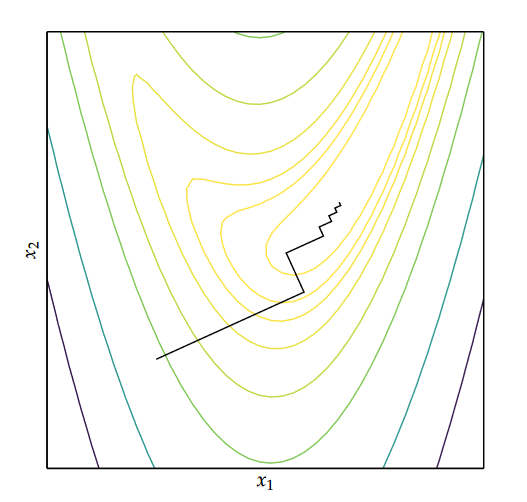
\includegraphics[width=0.5\textwidth]{gradientdescent.png}
        \caption{Source: \href{https://mitpress.mit.edu/9780262039420/}{Kochenderfer and Wheeler (2019)}}
        \end{figure}

    \end{frame}  

    \begin{frame}{Newton's method with line search}
        \begin{itemize}
            \item Recall that Newton's method is the iterative scheme: $$\bm{x}^{k+1} = \bm{x}^k - \mathbf{H}\of{\bm{x}^k}^{-1} \bp{\nabla f\of{\bm{x}^k}}^\intercal.$$
            \item This is a special case of the direction set method with 
            \begin{align*}
                \bm{s}^k = - \mathbf{H}\of{\bm{x}^k}^{-1} \bp{\nabla f\of{\bm{x}^k}}^\intercal \quad \text{and} \quad \lambda=1.
            \end{align*}
            \item But we can choose $\lambda$ to minimize $f\bp{\bm{x}^k + \lambda \bm{s}^k}$.
            \item Guaranteed to descend, but converges slower that Newton's method.
            \end{itemize}

    \end{frame}

    \begin{frame}{Quasi-Newton methods}
        \begin{itemize}
            \item Instead of using the exact Hessian, use some other  positive definite matrix -- easier to compute.
            \item One popular choice is the \alg{Broyden-Fletcher-Goldfarb-Shanno} (BFGS) method.
            \item Given some initial positive definite Hessian approximation $H_0$, the iterative scheme generates a sequence of positive definite matrices.
            \item One possibility: set $H_0$ to the identity matrix.
            \item Another possibility: set $H_0$ to the Hessian of the objective function at the initial point.
            \item No need to compute the true Hessian in each iteration.
            \end{itemize}
    \end{frame} 
    
    \begin{frame}{Trust region}
        \begin{itemize}
            \item First we set the maximum step size: \al{trust region} $\Delta_k$.
            \item We construct a quadratic approximation $m_k$ of the objective function around $\bm{x}^k$: we "trust" this approximation is good in the trust region around $\bm{x}^k$:
            $$m_k\bp{\bm{p}} = f\bp{\bm{x}^k} + \nabla f\bp{\bm{x}^k}^\intercal \bm{p} + \frac{1}{2} \bm{p}^\intercal \mathbf{H}_k \bm{p}$$ where $\mathbf{H}_k$ is a positive definite matrix:
            \item Find the minimum of $m_k$ in the trust region: $\bm{p}^k$.
            \item Set $\bm{x}^{k+1} = \bm{x}^k + \bm{p}^k$ if $f\bp{\bm{x}^{k+1}}<f\bp{\bm{x}^k}$.
            \item Trust region increased if the approximation was good, decreased otherwise.
            \end{itemize}
        \end{frame}   

        \begin{frame}{Trust region}
            \centering
            \begin{figure}
    
            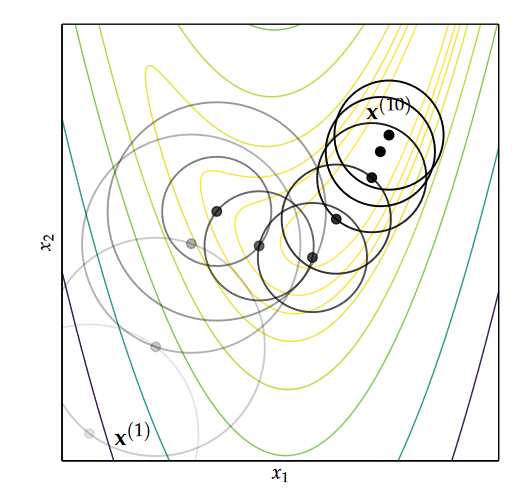
\includegraphics[width=0.50\textwidth]{trustregion.png}
            \caption{Source: \href{https://mitpress.mit.edu/9780262039420/}{Kochenderfer and Wheeler (2019)}}
            \end{figure}
    
        \end{frame}  

        \begin{frame}
            \heading{Constrained optimization}
        \end{frame}

        \begin{frame}{Overview}
            \begin{itemize}
                \item Constrained optimization \al{much more difficult} than unconstrained optimization.
                \begin{itemize}
                    \item Sometimes we can solve the problem by converting it to an unconstrained problem.
                \end{itemize}
                \item \al{Penalty methods}: convert constrained problem to an unconstrained problem (by adding a penalty term to the objective function).
                \item \alb{Sequential quadratic programming}: approximate the objective function by a quadratic and constraints by linear functions.
                \item \alg{Active set methods}: consider easier subproblems with only a subset of constraints binding.
                \item Key takeaway: \alr{do not} try to implement these methods yourself. Use existing packages.
                \end{itemize}
            \end{frame}   
\end{document}